


% Header, overrides base

    % Make sure that the sphinx doc style knows who it inherits from.
    \def\sphinxdocclass{article}

    % Declare the document class
    \documentclass[letterpaper,10pt,english]{/Users/madeleineudell/anaconda/lib/python2.7/site-packages/sphinx/texinputs/sphinxhowto}

    % Imports
    \usepackage[utf8]{inputenc}
    \DeclareUnicodeCharacter{00A0}{\\nobreakspace}
    \usepackage[T1]{fontenc}
    \usepackage{babel}
    \usepackage{times}
    \usepackage{import}
    \usepackage[Bjarne]{/Users/madeleineudell/anaconda/lib/python2.7/site-packages/sphinx/texinputs/fncychap}
    \usepackage{longtable}
    \usepackage{/Users/madeleineudell/anaconda/lib/python2.7/site-packages/sphinx/texinputs/sphinx}
    \usepackage{multirow}

    \usepackage{amsmath}
    \usepackage{amssymb}
    \usepackage{ucs}
    \usepackage{enumerate}

    % Used to make the Input/Output rules follow around the contents.
    \usepackage{needspace}

    % Pygments requirements
    \usepackage{fancyvrb}
    \usepackage{color}
    % ansi colors additions
    \definecolor{darkgreen}{rgb}{.12,.54,.11}
    \definecolor{lightgray}{gray}{.95}
    \definecolor{brown}{rgb}{0.54,0.27,0.07}
    \definecolor{purple}{rgb}{0.5,0.0,0.5}
    \definecolor{darkgray}{gray}{0.25}
    \definecolor{lightred}{rgb}{1.0,0.39,0.28}
    \definecolor{lightgreen}{rgb}{0.48,0.99,0.0}
    \definecolor{lightblue}{rgb}{0.53,0.81,0.92}
    \definecolor{lightpurple}{rgb}{0.87,0.63,0.87}
    \definecolor{lightcyan}{rgb}{0.5,1.0,0.83}

    % Needed to box output/input
    \usepackage{tikz}
        \usetikzlibrary{calc,arrows,shadows}
    \usepackage[framemethod=tikz]{mdframed}

    \usepackage{alltt}

    % Used to load and display graphics
    \usepackage{graphicx}
    \graphicspath{ {figs/} }
    \usepackage[Export]{adjustbox} % To resize

    % used so that images for notebooks which have spaces in the name can still be included
    \usepackage{grffile}


    % For formatting output while also word wrapping.
    \usepackage{listings}
    \lstset{breaklines=true}
    \lstset{basicstyle=\small\ttfamily}
    \def\smaller{\fontsize{9.5pt}{9.5pt}\selectfont}

    %Pygments definitions
    
\makeatletter
\def\PY@reset{\let\PY@it=\relax \let\PY@bf=\relax%
    \let\PY@ul=\relax \let\PY@tc=\relax%
    \let\PY@bc=\relax \let\PY@ff=\relax}
\def\PY@tok#1{\csname PY@tok@#1\endcsname}
\def\PY@toks#1+{\ifx\relax#1\empty\else%
    \PY@tok{#1}\expandafter\PY@toks\fi}
\def\PY@do#1{\PY@bc{\PY@tc{\PY@ul{%
    \PY@it{\PY@bf{\PY@ff{#1}}}}}}}
\def\PY#1#2{\PY@reset\PY@toks#1+\relax+\PY@do{#2}}

\expandafter\def\csname PY@tok@gd\endcsname{\def\PY@tc##1{\textcolor[rgb]{0.63,0.00,0.00}{##1}}}
\expandafter\def\csname PY@tok@gu\endcsname{\let\PY@bf=\textbf\def\PY@tc##1{\textcolor[rgb]{0.50,0.00,0.50}{##1}}}
\expandafter\def\csname PY@tok@gt\endcsname{\def\PY@tc##1{\textcolor[rgb]{0.00,0.27,0.87}{##1}}}
\expandafter\def\csname PY@tok@gs\endcsname{\let\PY@bf=\textbf}
\expandafter\def\csname PY@tok@gr\endcsname{\def\PY@tc##1{\textcolor[rgb]{1.00,0.00,0.00}{##1}}}
\expandafter\def\csname PY@tok@cm\endcsname{\let\PY@it=\textit\def\PY@tc##1{\textcolor[rgb]{0.25,0.50,0.50}{##1}}}
\expandafter\def\csname PY@tok@vg\endcsname{\def\PY@tc##1{\textcolor[rgb]{0.10,0.09,0.49}{##1}}}
\expandafter\def\csname PY@tok@m\endcsname{\def\PY@tc##1{\textcolor[rgb]{0.40,0.40,0.40}{##1}}}
\expandafter\def\csname PY@tok@mh\endcsname{\def\PY@tc##1{\textcolor[rgb]{0.40,0.40,0.40}{##1}}}
\expandafter\def\csname PY@tok@go\endcsname{\def\PY@tc##1{\textcolor[rgb]{0.53,0.53,0.53}{##1}}}
\expandafter\def\csname PY@tok@ge\endcsname{\let\PY@it=\textit}
\expandafter\def\csname PY@tok@vc\endcsname{\def\PY@tc##1{\textcolor[rgb]{0.10,0.09,0.49}{##1}}}
\expandafter\def\csname PY@tok@il\endcsname{\def\PY@tc##1{\textcolor[rgb]{0.40,0.40,0.40}{##1}}}
\expandafter\def\csname PY@tok@cs\endcsname{\let\PY@it=\textit\def\PY@tc##1{\textcolor[rgb]{0.25,0.50,0.50}{##1}}}
\expandafter\def\csname PY@tok@cp\endcsname{\def\PY@tc##1{\textcolor[rgb]{0.74,0.48,0.00}{##1}}}
\expandafter\def\csname PY@tok@gi\endcsname{\def\PY@tc##1{\textcolor[rgb]{0.00,0.63,0.00}{##1}}}
\expandafter\def\csname PY@tok@gh\endcsname{\let\PY@bf=\textbf\def\PY@tc##1{\textcolor[rgb]{0.00,0.00,0.50}{##1}}}
\expandafter\def\csname PY@tok@ni\endcsname{\let\PY@bf=\textbf\def\PY@tc##1{\textcolor[rgb]{0.60,0.60,0.60}{##1}}}
\expandafter\def\csname PY@tok@nl\endcsname{\def\PY@tc##1{\textcolor[rgb]{0.63,0.63,0.00}{##1}}}
\expandafter\def\csname PY@tok@nn\endcsname{\let\PY@bf=\textbf\def\PY@tc##1{\textcolor[rgb]{0.00,0.00,1.00}{##1}}}
\expandafter\def\csname PY@tok@no\endcsname{\def\PY@tc##1{\textcolor[rgb]{0.53,0.00,0.00}{##1}}}
\expandafter\def\csname PY@tok@na\endcsname{\def\PY@tc##1{\textcolor[rgb]{0.49,0.56,0.16}{##1}}}
\expandafter\def\csname PY@tok@nb\endcsname{\def\PY@tc##1{\textcolor[rgb]{0.00,0.50,0.00}{##1}}}
\expandafter\def\csname PY@tok@nc\endcsname{\let\PY@bf=\textbf\def\PY@tc##1{\textcolor[rgb]{0.00,0.00,1.00}{##1}}}
\expandafter\def\csname PY@tok@nd\endcsname{\def\PY@tc##1{\textcolor[rgb]{0.67,0.13,1.00}{##1}}}
\expandafter\def\csname PY@tok@ne\endcsname{\let\PY@bf=\textbf\def\PY@tc##1{\textcolor[rgb]{0.82,0.25,0.23}{##1}}}
\expandafter\def\csname PY@tok@nf\endcsname{\def\PY@tc##1{\textcolor[rgb]{0.00,0.00,1.00}{##1}}}
\expandafter\def\csname PY@tok@si\endcsname{\let\PY@bf=\textbf\def\PY@tc##1{\textcolor[rgb]{0.73,0.40,0.53}{##1}}}
\expandafter\def\csname PY@tok@s2\endcsname{\def\PY@tc##1{\textcolor[rgb]{0.73,0.13,0.13}{##1}}}
\expandafter\def\csname PY@tok@vi\endcsname{\def\PY@tc##1{\textcolor[rgb]{0.10,0.09,0.49}{##1}}}
\expandafter\def\csname PY@tok@nt\endcsname{\let\PY@bf=\textbf\def\PY@tc##1{\textcolor[rgb]{0.00,0.50,0.00}{##1}}}
\expandafter\def\csname PY@tok@nv\endcsname{\def\PY@tc##1{\textcolor[rgb]{0.10,0.09,0.49}{##1}}}
\expandafter\def\csname PY@tok@s1\endcsname{\def\PY@tc##1{\textcolor[rgb]{0.73,0.13,0.13}{##1}}}
\expandafter\def\csname PY@tok@sh\endcsname{\def\PY@tc##1{\textcolor[rgb]{0.73,0.13,0.13}{##1}}}
\expandafter\def\csname PY@tok@sc\endcsname{\def\PY@tc##1{\textcolor[rgb]{0.73,0.13,0.13}{##1}}}
\expandafter\def\csname PY@tok@sx\endcsname{\def\PY@tc##1{\textcolor[rgb]{0.00,0.50,0.00}{##1}}}
\expandafter\def\csname PY@tok@bp\endcsname{\def\PY@tc##1{\textcolor[rgb]{0.00,0.50,0.00}{##1}}}
\expandafter\def\csname PY@tok@c1\endcsname{\let\PY@it=\textit\def\PY@tc##1{\textcolor[rgb]{0.25,0.50,0.50}{##1}}}
\expandafter\def\csname PY@tok@kc\endcsname{\let\PY@bf=\textbf\def\PY@tc##1{\textcolor[rgb]{0.00,0.50,0.00}{##1}}}
\expandafter\def\csname PY@tok@c\endcsname{\let\PY@it=\textit\def\PY@tc##1{\textcolor[rgb]{0.25,0.50,0.50}{##1}}}
\expandafter\def\csname PY@tok@mf\endcsname{\def\PY@tc##1{\textcolor[rgb]{0.40,0.40,0.40}{##1}}}
\expandafter\def\csname PY@tok@err\endcsname{\def\PY@bc##1{\setlength{\fboxsep}{0pt}\fcolorbox[rgb]{1.00,0.00,0.00}{1,1,1}{\strut ##1}}}
\expandafter\def\csname PY@tok@kd\endcsname{\let\PY@bf=\textbf\def\PY@tc##1{\textcolor[rgb]{0.00,0.50,0.00}{##1}}}
\expandafter\def\csname PY@tok@ss\endcsname{\def\PY@tc##1{\textcolor[rgb]{0.10,0.09,0.49}{##1}}}
\expandafter\def\csname PY@tok@sr\endcsname{\def\PY@tc##1{\textcolor[rgb]{0.73,0.40,0.53}{##1}}}
\expandafter\def\csname PY@tok@mo\endcsname{\def\PY@tc##1{\textcolor[rgb]{0.40,0.40,0.40}{##1}}}
\expandafter\def\csname PY@tok@kn\endcsname{\let\PY@bf=\textbf\def\PY@tc##1{\textcolor[rgb]{0.00,0.50,0.00}{##1}}}
\expandafter\def\csname PY@tok@mi\endcsname{\def\PY@tc##1{\textcolor[rgb]{0.40,0.40,0.40}{##1}}}
\expandafter\def\csname PY@tok@gp\endcsname{\let\PY@bf=\textbf\def\PY@tc##1{\textcolor[rgb]{0.00,0.00,0.50}{##1}}}
\expandafter\def\csname PY@tok@o\endcsname{\def\PY@tc##1{\textcolor[rgb]{0.40,0.40,0.40}{##1}}}
\expandafter\def\csname PY@tok@kr\endcsname{\let\PY@bf=\textbf\def\PY@tc##1{\textcolor[rgb]{0.00,0.50,0.00}{##1}}}
\expandafter\def\csname PY@tok@s\endcsname{\def\PY@tc##1{\textcolor[rgb]{0.73,0.13,0.13}{##1}}}
\expandafter\def\csname PY@tok@kp\endcsname{\def\PY@tc##1{\textcolor[rgb]{0.00,0.50,0.00}{##1}}}
\expandafter\def\csname PY@tok@w\endcsname{\def\PY@tc##1{\textcolor[rgb]{0.73,0.73,0.73}{##1}}}
\expandafter\def\csname PY@tok@kt\endcsname{\def\PY@tc##1{\textcolor[rgb]{0.69,0.00,0.25}{##1}}}
\expandafter\def\csname PY@tok@ow\endcsname{\let\PY@bf=\textbf\def\PY@tc##1{\textcolor[rgb]{0.67,0.13,1.00}{##1}}}
\expandafter\def\csname PY@tok@sb\endcsname{\def\PY@tc##1{\textcolor[rgb]{0.73,0.13,0.13}{##1}}}
\expandafter\def\csname PY@tok@k\endcsname{\let\PY@bf=\textbf\def\PY@tc##1{\textcolor[rgb]{0.00,0.50,0.00}{##1}}}
\expandafter\def\csname PY@tok@se\endcsname{\let\PY@bf=\textbf\def\PY@tc##1{\textcolor[rgb]{0.73,0.40,0.13}{##1}}}
\expandafter\def\csname PY@tok@sd\endcsname{\let\PY@it=\textit\def\PY@tc##1{\textcolor[rgb]{0.73,0.13,0.13}{##1}}}

\def\PYZbs{\char`\\}
\def\PYZus{\char`\_}
\def\PYZob{\char`\{}
\def\PYZcb{\char`\}}
\def\PYZca{\char`\^}
\def\PYZam{\char`\&}
\def\PYZlt{\char`\<}
\def\PYZgt{\char`\>}
\def\PYZsh{\char`\#}
\def\PYZpc{\char`\%}
\def\PYZdl{\char`\$}
\def\PYZhy{\char`\-}
\def\PYZsq{\char`\'}
\def\PYZdq{\char`\"}
\def\PYZti{\char`\~}
% for compatibility with earlier versions
\def\PYZat{@}
\def\PYZlb{[}
\def\PYZrb{]}
\makeatother


    %Set pygments styles if needed...
    
        \definecolor{nbframe-border}{rgb}{0.867,0.867,0.867}
        \definecolor{nbframe-bg}{rgb}{0.969,0.969,0.969}
        \definecolor{nbframe-in-prompt}{rgb}{0.0,0.0,0.502}
        \definecolor{nbframe-out-prompt}{rgb}{0.545,0.0,0.0}

        \newenvironment{ColorVerbatim}
        {\begin{mdframed}[%
            roundcorner=1.0pt, %
            backgroundcolor=nbframe-bg, %
            userdefinedwidth=1\linewidth, %
            leftmargin=0.1\linewidth, %
            innerleftmargin=0pt, %
            innerrightmargin=0pt, %
            linecolor=nbframe-border, %
            linewidth=1pt, %
            usetwoside=false, %
            everyline=true, %
            innerlinewidth=3pt, %
            innerlinecolor=nbframe-bg, %
            middlelinewidth=1pt, %
            middlelinecolor=nbframe-bg, %
            outerlinewidth=0.5pt, %
            outerlinecolor=nbframe-border, %
            needspace=0pt
        ]}
        {\end{mdframed}}
        
        \newenvironment{InvisibleVerbatim}
        {\begin{mdframed}[leftmargin=0.1\linewidth,innerleftmargin=3pt,innerrightmargin=3pt, userdefinedwidth=1\linewidth, linewidth=0pt, linecolor=white, usetwoside=false]}
        {\end{mdframed}}

        \renewenvironment{Verbatim}[1][\unskip]
        {\begin{alltt}\smaller}
        {\end{alltt}}
    

    % Help prevent overflowing lines due to urls and other hard-to-break 
    % entities.  This doesn't catch everything...
    \sloppy

    % Document level variables
    \title{quickstart}
    \date{August 21, 2013}
    \release{}
    \author{Unknown Author}
    \renewcommand{\releasename}{}

    % TODO: Add option for the user to specify a logo for his/her export.
    \newcommand{\sphinxlogo}{}

    % Make the index page of the document.
    \makeindex

    % Import sphinx document type specifics.
     


% Body

    % Start of the document
    \begin{document}

        
            \maketitle
        

        


        
        title: SIGOPT: a python package for sigmoidal programming author:
Madeleine Udell

\section{SIGOPT: a python package for sigmoidal programming}

SIGOPT is a python package for solving sigmoidal programming problems of
the following form:

\[
\begin{array}{ll} 
\mbox{\textrm{maximize}} & \sum_{i=1}^n f_i(x_i) \\ 
\mbox{subject to} & Ax \leq b, \\
& Cx = d, \\
& l \leq x \leq u,
\end{array}
\]

where $A,b,C,d,l,u$ are matrices or lists of the appropriate dimensions,
and $f_i$, $i=1,\ldots,k$ are \emph{sigmoidal} functions. $f_i$ is
\emph{sigmoidal} if it is \emph{convex} on the interval $[l_i,z_i]$, and
\emph{concave} on the interval $[z_i,u_i]$.

(It's ok if $l_i=z_i$ or $z_i=u_i$, so $f_i$ can be just convex or just
concave.)

To understand how SIGOPT works, and to learn more about the theory of
sigmoidal programming, you can take a look at
\href{www.stanford.edu/~udell/doc/max_sum_sigmoids.pdf}{this paper}.

To learn more about how to use SIGOPT, read on.\section{Download}

SIGOPT is available via the
\href{https://pypi.python.org/pypi?\%3Aaction=search\&term=sigopt\&submit=search}{python
package index}. You can install it using \texttt{easy\_install}

\begin{verbatim}
$ easy_install sigopt
\end{verbatim}

or \texttt{pip}

\begin{verbatim}
$ pip install sigopt
\end{verbatim}

Or the old-fashioned way: download it from
\href{https://pypi.python.org/pypi?\%3Aaction=search\&term=sigopt\&submit=search}{PyPI},
unzip the package, and install:

\begin{verbatim}
$ python setup.py install
\end{verbatim}

\subsection{Dependencies}

Before SIGOPT will work, you'll need to install the
\href{http://www.gnu.org/software/glpk/}{GNU Linear Programming Kit
(GLPK)}. Make sure to install GLPK in a standard location so that PyGLPK
can find it.

With the exception of GLPK, all of the dependencies are available via
the \href{https://pypi.python.org}{python package index}, and are
automatically downloaded and installed if they are not already found on
the system.

\begin{itemize}
\itemsep1pt\parskip0pt\parsep0pt
\item
  PyGLPK
\item
  cvxopt
\item
  numpy
\item
  scipy
\item
  matplotlib
\end{itemize}\section{Quickstart examples}

\subsection{A simple sigmoidal program}

As an example to get you started, we'll show how to solve the problem

\[
\begin{array}{ll}
\mbox{\textrm{maximize}} & \sum_{i=1}^9 \mathop{logistic}(x_i) \\
\mbox{subject to} & \sum_i x_i \leq 0, \\
& -5 \leq x \leq 5.
\end{array}
\]

Each function $f_i$ is specified as a tuple consisting of the function,
its derivative, and its inflection point $z_i$.

The logistic function $\mathop{logistic}(x) = 1/\exp(-x)$ and its
derivative are defined for convenience in \texttt{sigopt.functions}, and
its inflection point is located at $z=0$.

    % Make sure that atleast 4 lines are below the HR
    \needspace{4\baselineskip}

    
        \vspace{6pt}
        \makebox[0.1\linewidth]{\smaller\hfill\tt\color{nbframe-in-prompt}In\hspace{4pt}{[}1{]}:\hspace{4pt}}\\*
        \vspace{-2.65\baselineskip}
        \begin{ColorVerbatim}
            \vspace{-0.7\baselineskip}
            \begin{Verbatim}[commandchars=\\\{\}]
\PY{k+kn}{import} \PY{n+nn}{sigopt}
\PY{k+kn}{from} \PY{n+nn}{sigopt.functions} \PY{k+kn}{import} \PY{n}{logistic}\PY{p}{,} \PY{n}{logistic\PYZus{}prime}

\PY{c}{\PYZsh{} define f\PYZus{}i}
\PY{n}{fi} \PY{o}{=} \PY{p}{[}\PY{p}{(}\PY{n}{logistic}\PY{p}{,} \PY{n}{logistic\PYZus{}prime}\PY{p}{,} \PY{l+m+mi}{0}\PY{p}{)}\PY{p}{]}
\PY{c}{\PYZsh{} each f is identical, so we just repeat f\PYZus{}i 9 times}
\PY{n}{n} \PY{o}{=} \PY{l+m+mi}{9}
\PY{n}{fs} \PY{o}{=} \PY{n}{fi}\PY{o}{*}\PY{n}{n}
\end{Verbatim}

            
                \vspace{-0.2\baselineskip}
            
        \end{ColorVerbatim}
    
We write the constraint $\sum_i x_i \leq 0$ as $Ax \leq b$

    % Make sure that atleast 4 lines are below the HR
    \needspace{4\baselineskip}

    
        \vspace{6pt}
        \makebox[0.1\linewidth]{\smaller\hfill\tt\color{nbframe-in-prompt}In\hspace{4pt}{[}2{]}:\hspace{4pt}}\\*
        \vspace{-2.65\baselineskip}
        \begin{ColorVerbatim}
            \vspace{-0.7\baselineskip}
            \begin{Verbatim}[commandchars=\\\{\}]
\PY{n}{A} \PY{o}{=} \PY{n}{numpy}\PY{o}{.}\PY{n}{ones}\PY{p}{(}\PY{p}{(}\PY{l+m+mi}{1}\PY{p}{,}\PY{n}{n}\PY{p}{)}\PY{p}{)}
\PY{n}{b} \PY{o}{=} \PY{n}{numpy}\PY{o}{.}\PY{n}{ones}\PY{p}{(}\PY{p}{(}\PY{l+m+mi}{1}\PY{p}{,}\PY{l+m+mi}{1}\PY{p}{)}\PY{p}{)}
\end{Verbatim}

            
                \vspace{-0.2\baselineskip}
            
        \end{ColorVerbatim}
    
and the box constraints $l \leq x \leq u$ are

    % Make sure that atleast 4 lines are below the HR
    \needspace{4\baselineskip}

    
        \vspace{6pt}
        \makebox[0.1\linewidth]{\smaller\hfill\tt\color{nbframe-in-prompt}In\hspace{4pt}{[}3{]}:\hspace{4pt}}\\*
        \vspace{-2.65\baselineskip}
        \begin{ColorVerbatim}
            \vspace{-0.7\baselineskip}
            \begin{Verbatim}[commandchars=\\\{\}]
\PY{n}{l} \PY{o}{=} \PY{p}{[}\PY{o}{\PYZhy{}}\PY{l+m+mi}{5}\PY{p}{]}\PY{o}{*}\PY{n}{n}
\PY{n}{u} \PY{o}{=} \PY{p}{[}\PY{l+m+mi}{5}\PY{p}{]}\PY{o}{*}\PY{n}{n}
\end{Verbatim}

            
                \vspace{-0.2\baselineskip}
            
        \end{ColorVerbatim}
    
(these can be expressed either using numpy matrices, numpy arrays, or
python lists --- actually, anything iterable will do).

Now we're ready to formulate the problem

    % Make sure that atleast 4 lines are below the HR
    \needspace{4\baselineskip}

    
        \vspace{6pt}
        \makebox[0.1\linewidth]{\smaller\hfill\tt\color{nbframe-in-prompt}In\hspace{4pt}{[}4{]}:\hspace{4pt}}\\*
        \vspace{-2.65\baselineskip}
        \begin{ColorVerbatim}
            \vspace{-0.7\baselineskip}
            \begin{Verbatim}[commandchars=\\\{\}]
\PY{k+kn}{from} \PY{n+nn}{sigopt} \PY{k+kn}{import} \PY{n}{Problem}
\PY{n}{p} \PY{o}{=} \PY{n}{Problem}\PY{p}{(}\PY{n}{l}\PY{p}{,}\PY{n}{u}\PY{p}{,}\PY{n}{fs}\PY{p}{,}\PY{n}{A}\PY{o}{=}\PY{n}{A}\PY{p}{,}\PY{n}{b}\PY{o}{=}\PY{n}{b}\PY{p}{,}\PY{n}{name}\PY{o}{=}\PY{l+s}{\PYZsq{}}\PY{l+s}{example1}\PY{l+s}{\PYZsq{}}\PY{p}{,}\PY{n}{tol}\PY{o}{=}\PY{o}{.}\PY{l+m+mi}{1}\PY{p}{,}\PY{n}{sub\PYZus{}tol}\PY{o}{=}\PY{o}{.}\PY{l+m+mo}{01}\PY{p}{)}
\end{Verbatim}

            
                \vspace{-0.2\baselineskip}
            
        \end{ColorVerbatim}
    
The parameter \texttt{tol} sets the accuracy to which we need to solve
the problem, and \texttt{sub\_tol} controls the quality of the upper
approximation to the functions $f_i$. Finally we solve!

    % Make sure that atleast 4 lines are below the HR
    \needspace{4\baselineskip}

    
        \vspace{6pt}
        \makebox[0.1\linewidth]{\smaller\hfill\tt\color{nbframe-in-prompt}In\hspace{4pt}{[}5{]}:\hspace{4pt}}\\*
        \vspace{-2.65\baselineskip}
        \begin{ColorVerbatim}
            \vspace{-0.7\baselineskip}
            \begin{Verbatim}[commandchars=\\\{\}]
\PY{n}{p}\PY{o}{.}\PY{n}{solve}\PY{p}{(}\PY{n}{maxiters} \PY{o}{=} \PY{l+m+mi}{100}\PY{p}{)}
\end{Verbatim}

            
                \vspace{-0.2\baselineskip}
            
        \end{ColorVerbatim}
    
(It's a good idea to specify a maximum number of iterations, since
sigmoidal programs can me NP-hard.)

We can examine the bounds on the optimal value, and the point $x$
achieving those bounds.

    % Make sure that atleast 4 lines are below the HR
    \needspace{4\baselineskip}

    
        \vspace{6pt}
        \makebox[0.1\linewidth]{\smaller\hfill\tt\color{nbframe-in-prompt}In\hspace{4pt}{[}6{]}:\hspace{4pt}}\\*
        \vspace{-2.65\baselineskip}
        \begin{ColorVerbatim}
            \vspace{-0.7\baselineskip}
            \begin{Verbatim}[commandchars=\\\{\}]
\PY{k}{print} \PY{l+s}{\PYZsq{}}\PY{l+s}{bounds}\PY{l+s}{\PYZsq{}}\PY{p}{,}\PY{n}{p}\PY{o}{.}\PY{n}{bounds}
\PY{k}{print} \PY{l+s}{\PYZsq{}}\PY{l+s}{solution}\PY{l+s}{\PYZsq{}}\PY{p}{,}\PY{n}{p}\PY{o}{.}\PY{n}{x}
\end{Verbatim}

            
                \vspace{-0.2\baselineskip}
            
        \end{ColorVerbatim}
    

    

        % If the first block is an image, minipage the image.  Else
        % request a certain amount of space for the input text.
        \needspace{4\baselineskip}
        
        

            % Add document contents.
            
                \begin{InvisibleVerbatim}
                \vspace{-0.5\baselineskip}
\begin{alltt}bounds [(5.514779744166213, 5.820557154787409), (5.514779744166213,
5.823791589918229), (5.520849002950583, 5.828114180032125),
(5.546101925223407, 5.83318656497994), (5.601172194820388,
5.838282831707601), (5.6870586416451, 5.842525542312434),
(5.770608770092042, 5.846244704731432)]
solution [0.8001359691991636, 1.5064185015401645, 1.5438259874988653,
1.645357260519695, 1.7503615765704392, 1.8404877155833232,
1.9134129890883498, -5.0, -5.0]
\end{alltt}

            \end{InvisibleVerbatim}
            
        
    
Of course, it's nicer to see what's going on in a picture. We can plot
the best solution we've found so far using the plotting library.

    % Make sure that atleast 4 lines are below the HR
    \needspace{4\baselineskip}

    
        \vspace{6pt}
        \makebox[0.1\linewidth]{\smaller\hfill\tt\color{nbframe-in-prompt}In\hspace{4pt}{[}7{]}:\hspace{4pt}}\\*
        \vspace{-2.65\baselineskip}
        \begin{ColorVerbatim}
            \vspace{-0.7\baselineskip}
            \begin{Verbatim}[commandchars=\\\{\}]
\PY{k+kn}{from} \PY{n+nn}{sigopt.plot} \PY{k+kn}{import} \PY{o}{*}
\PY{n}{f} \PY{o}{=} \PY{n}{plot\PYZus{}best\PYZus{}node}\PY{p}{(}\PY{n}{p}\PY{p}{)}
\PY{n}{f}\PY{o}{.}\PY{n}{show}\PY{p}{(}\PY{p}{)}
\end{Verbatim}

            
                \vspace{-0.2\baselineskip}
            
        \end{ColorVerbatim}
    

    

        % If the first block is an image, minipage the image.  Else
        % request a certain amount of space for the input text.
        \needspace{4\baselineskip}
        
        

            % Add document contents.
            
                \begin{InvisibleVerbatim}
                \vspace{-0.5\baselineskip}
\begin{alltt}Saving figure in example1\_best\_node.eps
\end{alltt}

            \end{InvisibleVerbatim}
            
                \begin{InvisibleVerbatim}
                \vspace{-0.5\baselineskip}
\begin{alltt}/Users/Madeleine/Applications/anaconda/lib/python2.7/site-
packages/matplotlib/figure.py:361: UserWarning: matplotlib is
currently using a non-GUI backend, so cannot show the figure
  "matplotlib is currently using a non-GUI backend, "
\end{alltt}

            \end{InvisibleVerbatim}
            
                \begin{InvisibleVerbatim}
                \vspace{-0.5\baselineskip}
    \begin{center}
    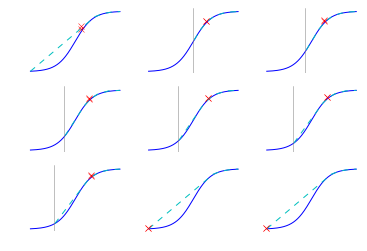
\includegraphics[max size={\textwidth}{\textheight}]{quickstart_files/quickstart_15_2.png}
    \par
    \end{center}
    
            \end{InvisibleVerbatim}
            
        
    
And if we'd like to see how quickly the algorithm converged, there's a
convenient convergence plot.

    % Make sure that atleast 4 lines are below the HR
    \needspace{4\baselineskip}

    
        \vspace{6pt}
        \makebox[0.1\linewidth]{\smaller\hfill\tt\color{nbframe-in-prompt}In\hspace{4pt}{[}8{]}:\hspace{4pt}}\\*
        \vspace{-2.65\baselineskip}
        \begin{ColorVerbatim}
            \vspace{-0.7\baselineskip}
            \begin{Verbatim}[commandchars=\\\{\}]
\PY{n}{f} \PY{o}{=} \PY{n}{plot\PYZus{}convergence}\PY{p}{(}\PY{n}{p}\PY{p}{)}
\PY{n}{f}\PY{o}{.}\PY{n}{show}\PY{p}{(}\PY{p}{)}
\end{Verbatim}

            
                \vspace{-0.2\baselineskip}
            
        \end{ColorVerbatim}
    

    

        % If the first block is an image, minipage the image.  Else
        % request a certain amount of space for the input text.
        \needspace{4\baselineskip}
        
        

            % Add document contents.
            
                \begin{InvisibleVerbatim}
                \vspace{-0.5\baselineskip}
\begin{alltt}Saving plot of history in example1\_convergence.eps
\end{alltt}

            \end{InvisibleVerbatim}
            
                \begin{InvisibleVerbatim}
                \vspace{-0.5\baselineskip}
    \begin{center}
    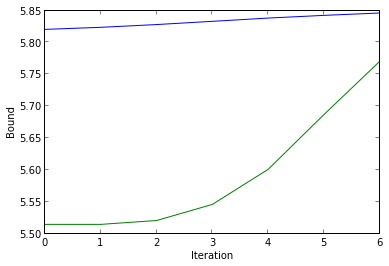
\includegraphics[max size={\textwidth}{\textheight}]{quickstart_files/quickstart_17_1.png}
    \par
    \end{center}
    
            \end{InvisibleVerbatim}
            
        
    
\subsection{Function definitions, equality and inequality constraints}

We can also define our own functions using the full power of python. For
example,

    % Make sure that atleast 4 lines are below the HR
    \needspace{4\baselineskip}

    
        \vspace{6pt}
        \makebox[0.1\linewidth]{\smaller\hfill\tt\color{nbframe-in-prompt}In\hspace{4pt}{[}9{]}:\hspace{4pt}}\\*
        \vspace{-2.65\baselineskip}
        \begin{ColorVerbatim}
            \vspace{-0.7\baselineskip}
            \begin{Verbatim}[commandchars=\\\{\}]
\PY{k+kn}{import} \PY{n+nn}{math}

\PY{c}{\PYZsh{} my crazy sigmoidal function}
\PY{k}{def} \PY{n+nf}{crazy\PYZus{}sigmoid}\PY{p}{(}\PY{n}{x}\PY{p}{,}\PY{n}{param}\PY{p}{)}\PY{p}{:}
    \PY{k}{if} \PY{n}{x} \PY{o}{\PYZgt{}} \PY{n}{param}\PY{p}{:}
        \PY{k}{return} \PY{o}{\PYZhy{}}\PY{n}{math}\PY{o}{.}\PY{n}{pow}\PY{p}{(}\PY{n}{x} \PY{o}{\PYZhy{}} \PY{n}{param}\PY{p}{,}\PY{l+m+mi}{2}\PY{p}{)}
    \PY{k}{else}\PY{p}{:}
        \PY{k}{return} \PY{n}{math}\PY{o}{.}\PY{n}{pow}\PY{p}{(}\PY{n}{x} \PY{o}{\PYZhy{}} \PY{n}{param}\PY{p}{,}\PY{l+m+mi}{2}\PY{p}{)}
    
\PY{k}{def} \PY{n+nf}{crazy\PYZus{}sigmoid\PYZus{}prime}\PY{p}{(}\PY{n}{x}\PY{p}{,}\PY{n}{param}\PY{p}{)}\PY{p}{:}
    \PY{k}{if} \PY{n}{x} \PY{o}{\PYZgt{}} \PY{n}{param}\PY{p}{:}
        \PY{k}{return} \PY{o}{\PYZhy{}}\PY{l+m+mi}{2}\PY{o}{*}\PY{p}{(}\PY{n}{x} \PY{o}{\PYZhy{}} \PY{n}{param}\PY{p}{)}
    \PY{k}{else}\PY{p}{:}
        \PY{k}{return} \PY{l+m+mi}{2}\PY{o}{*}\PY{p}{(}\PY{n}{x} \PY{o}{\PYZhy{}} \PY{n}{param}\PY{p}{)}

\PY{n}{n} \PY{o}{=} \PY{l+m+mi}{9}
\PY{n}{crazy\PYZus{}fs} \PY{o}{=} \PY{p}{[}\PY{p}{(}\PY{k}{lambda} \PY{n}{x}\PY{p}{,} \PY{n}{p}\PY{o}{=}\PY{n}{p}\PY{p}{:} \PY{n}{crazy\PYZus{}sigmoid}\PY{p}{(}\PY{n}{x}\PY{p}{,}\PY{n}{p}\PY{p}{)}\PY{p}{,}
             \PY{k}{lambda} \PY{n}{x}\PY{p}{,} \PY{n}{p}\PY{o}{=}\PY{n}{p}\PY{p}{:} \PY{n}{crazy\PYZus{}sigmoid\PYZus{}prime}\PY{p}{(}\PY{n}{x}\PY{p}{,}\PY{n}{p}\PY{p}{)}\PY{p}{,}
             \PY{n}{p}\PY{p}{)} \PY{k}{for} \PY{n}{p} \PY{o+ow}{in} \PY{n+nb}{range}\PY{p}{(}\PY{n}{n}\PY{p}{)}\PY{p}{]}
\end{Verbatim}

            
                \vspace{-0.2\baselineskip}
            
        \end{ColorVerbatim}
    
Let's add a couple of equality and inequality constraints, and solve!

    % Make sure that atleast 4 lines are below the HR
    \needspace{4\baselineskip}

    
        \vspace{6pt}
        \makebox[0.1\linewidth]{\smaller\hfill\tt\color{nbframe-in-prompt}In\hspace{4pt}{[}10{]}:\hspace{4pt}}\\*
        \vspace{-2.65\baselineskip}
        \begin{ColorVerbatim}
            \vspace{-0.7\baselineskip}
            \begin{Verbatim}[commandchars=\\\{\}]
\PY{n}{k}\PY{p}{,}\PY{n}{m} \PY{o}{=} \PY{l+m+mi}{1}\PY{p}{,}\PY{l+m+mi}{2}
\PY{c}{\PYZsh{} inequality constraints Ax \PYZlt{}= b}
\PY{n}{A} \PY{o}{=} \PY{n}{numpy}\PY{o}{.}\PY{n}{random}\PY{o}{.}\PY{n}{normal}\PY{p}{(}\PY{l+m+mi}{0}\PY{p}{,}\PY{l+m+mi}{1}\PY{p}{,}\PY{p}{(}\PY{n}{m}\PY{p}{,}\PY{n}{n}\PY{p}{)}\PY{p}{)}
\PY{n}{b} \PY{o}{=} \PY{n}{numpy}\PY{o}{.}\PY{n}{random}\PY{o}{.}\PY{n}{uniform}\PY{p}{(}\PY{l+m+mi}{0}\PY{p}{,}\PY{l+m+mi}{2}\PY{p}{,}\PY{n}{m}\PY{p}{)}\PY{o}{\PYZhy{}}\PY{l+m+mi}{1}
\PY{c}{\PYZsh{} equality constraints Cx == d}
\PY{n}{C} \PY{o}{=} \PY{n}{numpy}\PY{o}{.}\PY{n}{random}\PY{o}{.}\PY{n}{normal}\PY{p}{(}\PY{l+m+mi}{0}\PY{p}{,}\PY{l+m+mi}{1}\PY{p}{,}\PY{p}{(}\PY{n}{k}\PY{p}{,}\PY{n}{n}\PY{p}{)}\PY{p}{)}
\PY{n}{d} \PY{o}{=} \PY{n}{numpy}\PY{o}{.}\PY{n}{random}\PY{o}{.}\PY{n}{uniform}\PY{p}{(}\PY{l+m+mi}{0}\PY{p}{,}\PY{l+m+mi}{2}\PY{p}{,}\PY{n}{k}\PY{p}{)}\PY{o}{\PYZhy{}}\PY{l+m+mi}{1}
\PY{c}{\PYZsh{} box constraints}
\PY{n}{l} \PY{o}{=} \PY{p}{[}\PY{o}{\PYZhy{}}\PY{l+m+mi}{10}\PY{p}{]}\PY{o}{*}\PY{n}{n}
\PY{n}{u} \PY{o}{=} \PY{p}{[}\PY{l+m+mi}{10}\PY{p}{]}\PY{o}{*}\PY{n}{n}

\PY{n}{p} \PY{o}{=} \PY{n}{Problem}\PY{p}{(}\PY{n}{l}\PY{p}{,}\PY{n}{u}\PY{p}{,}\PY{n}{crazy\PYZus{}fs}\PY{p}{,}\PY{n}{A}\PY{o}{=}\PY{n}{A}\PY{p}{,}\PY{n}{b}\PY{o}{=}\PY{n}{b}\PY{p}{,}\PY{n}{C}\PY{o}{=}\PY{n}{C}\PY{p}{,}\PY{n}{d}\PY{o}{=}\PY{n}{d}\PY{p}{,}\PY{n}{name}\PY{o}{=}\PY{l+s}{\PYZsq{}}\PY{l+s}{example2}\PY{l+s}{\PYZsq{}}\PY{p}{,}\PY{n}{tol}\PY{o}{=}\PY{o}{.}\PY{l+m+mi}{1}\PY{p}{,}\PY{n}{sub\PYZus{}tol}\PY{o}{=}\PY{o}{.}\PY{l+m+mo}{01}\PY{p}{)}
\PY{n}{p}\PY{o}{.}\PY{n}{solve}\PY{p}{(}\PY{n}{maxiters}\PY{o}{=}\PY{l+m+mi}{20}\PY{p}{)}
\PY{n}{f} \PY{o}{=} \PY{n}{plot\PYZus{}convergence}\PY{p}{(}\PY{n}{p}\PY{p}{)}
\PY{n}{f}\PY{o}{.}\PY{n}{show}\PY{p}{(}\PY{p}{)}
\end{Verbatim}

            
                \vspace{-0.2\baselineskip}
            
        \end{ColorVerbatim}
    

    

        % If the first block is an image, minipage the image.  Else
        % request a certain amount of space for the input text.
        \needspace{4\baselineskip}
        
        

            % Add document contents.
            
                \begin{InvisibleVerbatim}
                \vspace{-0.5\baselineskip}
\begin{alltt}Saving plot of history in example2\_convergence.eps
\end{alltt}

            \end{InvisibleVerbatim}
            
                \begin{InvisibleVerbatim}
                \vspace{-0.5\baselineskip}
    \begin{center}
    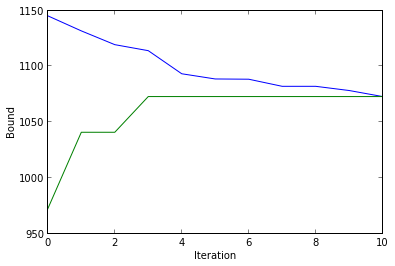
\includegraphics[max size={\textwidth}{\textheight}]{quickstart_files/quickstart_21_1.png}
    \par
    \end{center}
    
            \end{InvisibleVerbatim}
            
        
    
It looks like we've converged, so we'll take a look at the solution.

    % Make sure that atleast 4 lines are below the HR
    \needspace{4\baselineskip}

    
        \vspace{6pt}
        \makebox[0.1\linewidth]{\smaller\hfill\tt\color{nbframe-in-prompt}In\hspace{4pt}{[}11{]}:\hspace{4pt}}\\*
        \vspace{-2.65\baselineskip}
        \begin{ColorVerbatim}
            \vspace{-0.7\baselineskip}
            \begin{Verbatim}[commandchars=\\\{\}]
\PY{n}{f} \PY{o}{=} \PY{n}{plot\PYZus{}best\PYZus{}node}\PY{p}{(}\PY{n}{p}\PY{p}{)}
\PY{n}{f}\PY{o}{.}\PY{n}{show}\PY{p}{(}\PY{p}{)}
\end{Verbatim}

            
                \vspace{-0.2\baselineskip}
            
        \end{ColorVerbatim}
    

    

        % If the first block is an image, minipage the image.  Else
        % request a certain amount of space for the input text.
        \needspace{4\baselineskip}
        
        

            % Add document contents.
            
                \begin{InvisibleVerbatim}
                \vspace{-0.5\baselineskip}
\begin{alltt}Saving figure in example2\_best\_node.eps
\end{alltt}

            \end{InvisibleVerbatim}
            
                \begin{InvisibleVerbatim}
                \vspace{-0.5\baselineskip}
    \begin{center}
    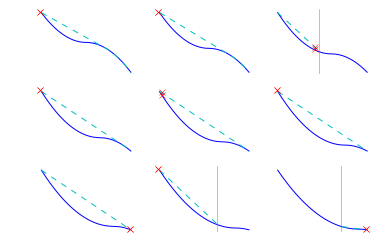
\includegraphics[max size={\textwidth}{\textheight}]{quickstart_files/quickstart_23_1.png}
    \par
    \end{center}
    
            \end{InvisibleVerbatim}
            
        
    
\section{More information}For more examples of how to use SIGOPT, consult the examples in
\texttt{sigopt.examples}. All functions are documented in their
docstrings as well.

To understand how SIGOPT works, and to learn more about the theory of
sigmoidal programming, you can take a look at
\href{www.stanford.edu/~udell/doc/max_sum_sigmoids.pdf}{this paper}.
        

        \renewcommand{\indexname}{Index}
        \printindex

    % End of document
    \end{document}


